% Choose one to switch between slides and handout
\documentclass[]{beamer}
%\documentclass[handout]{beamer}

% Video Meta Data
\title{Bitcoin, Blockchain and Cryptoassets}
\subtitle{Symmetric Cryptography}
\author{Prof. Dr. Fabian Schär}
\institute{University of Basel}

% Config File
% Packages
\usepackage[utf8]{inputenc}
\usepackage{hyperref}
\usepackage{gitinfo2}
\usepackage{tikz}
\usepackage{amsmath}
\usepackage{bibentry}
\usepackage{xcolor}
\usepackage{colortbl} % Add colour to LaTeX tables
\usepackage{caption}
\usepackage[export]{adjustbox}
\usepackage{pgfplots} \pgfplotsset{compat = 1.17}

% Color Options
\definecolor{highlight}{rgb}{0.65,0.84,0.82}
\definecolor{focus}{rgb}{0.72, 0, 0}

% Beamer Template Options
\beamertemplatenavigationsymbolsempty
\setbeamertemplate{footline}[frame number]
\setbeamercolor{structure}{fg=black}
\setbeamercolor{footline}{fg=black}
\setbeamercolor{title}{fg=black}
\setbeamercolor{frametitle}{fg=black}
\setbeamercolor{item}{fg=black}
\setbeamercolor{}{fg=black}
\setbeamercolor{bibliography item}{fg=black}
\setbeamercolor*{bibliography entry title}{fg=black}
\setbeamertemplate{items}[square]
\setbeamertemplate{enumerate items}[default]
\captionsetup[figure]{labelfont={color=black},font={color=black}}
\captionsetup[table]{labelfont={color=black},font={color=black}}

\setbeamertemplate{bibliography item}{\insertbiblabel}

% Link Icon Command
\newcommand{\link}{%
    \tikz[x=1.2ex, y=1.2ex, baseline=-0.05ex]{%
        \begin{scope}[x=1ex, y=1ex]
            \clip (-0.1,-0.1)
                --++ (-0, 1.2)
                --++ (0.6, 0)
                --++ (0, -0.6)
                --++ (0.6, 0)
                --++ (0, -1);
            \path[draw,
                line width = 0.5,
                rounded corners=0.5]
                (0,0) rectangle (1,1);
        \end{scope}
        \path[draw, line width = 0.5] (0.5, 0.5)
            -- (1, 1);
        \path[draw, line width = 0.5] (0.6, 1)
            -- (1, 1) -- (1, 0.6);
        }
    }

% Read Git Data from Github Actions Workflow
% Defaults to gitinfo2 for local builds
\IfFileExists{gitInfo.txt}
	{\input{gitInfo.txt}}
	{
		\newcommand{\gitRelease}{(Local Release)}
		\newcommand{\gitSHA}{\gitHash}
		\newcommand{\gitDate}{\gitAuthorIsoDate}
	}

% Custom Titlepage
\defbeamertemplate*{title page}{customized}[1][]
{
  \vspace{-0cm}\hfill
\includegraphics[width=2.5cm]{../config/logo_cif}
  
\includegraphics[width=1.9cm]{../config/seal_wwz}
  \\ \vspace{2em}
  \usebeamerfont{title}\textbf{\inserttitle}\par
  \usebeamerfont{title}\usebeamercolor[fg]{title}\insertsubtitle\par  \vspace{1.5em}
  \small\usebeamerfont{author}\insertauthor\par
  \usebeamerfont{author}\insertinstitute\par \vspace{2em}
  \usebeamercolor[fg]{titlegraphic}\inserttitlegraphic
    \tiny \noindent \texttt{Release Ver.: \gitRelease}\\ 
    \texttt{Version Hash: \gitSHA}\\
    \texttt{Version Date: \gitDate}\\ \vspace{1em}
  \link \href{https://github.com/cifunibas/Bitcoin-Blockchain-Cryptoassets/blob/main/slides/intro.pdf}
  {Get most recent version}\\
  \link \href{https://github.com/cifunibas/Bitcoin-Blockchain-Cryptoassets/blob/main/slides/intro.pdf}
  {Watch video lecture}\\ \vspace{1em}
  License: \texttt{Creative Commons Attribution-NonCommercial-ShareAlike 4.0 International}\\\vspace{2em}
  
\includegraphics[width = 1.2cm]{../config/license}
}

% tikzlibraries
\usetikzlibrary{decorations.pathreplacing}
\usetikzlibrary{decorations.markings}
\usetikzlibrary{positioning}

%caption font
\captionsetup{font=footnotesize}


%%%%%%%%%%%%%%%%%%%%%%%%%%%%%%%%%%%%%%%%%%%%%%
%%%%%%%%%%%%%%%%%%%%%%%%%%%%%%%%%%%%%%%%%%%%%%
\begin{document}

\thispagestyle{empty}
\begin{frame}[noframenumbering]
	\titlepage
\end{frame}
%%%

%%%
\begin{frame}{Types of Secret Writing}
	\begin{figure}
		\centering
		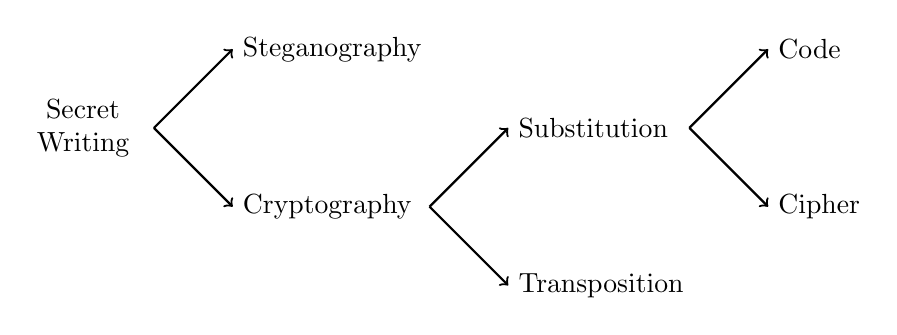
\begin{tikzpicture}[domain=1:10,scale=1]
			\coordinate (o1) at (1.9,6);
			\coordinate (t21) at (2.9,7); % txx:= target coordinate for arrow
			\coordinate (t22) at (2.9,5);
			\coordinate (o22) at (5.4,5); % oxx:= origin coordinate for arrow
			\coordinate (t31) at (6.4,6);
			\coordinate (t32) at (6.4,4);
			\coordinate (o31) at (8.7,6);
			\coordinate (t41) at (9.7,7);
			\coordinate (t42) at (9.7,5);
			
			\node[align=center] at (1,6) [] {Secret\\ Writing};
			\draw[color=black,thick, ->] (o1) to[] (t21) node[right]{Steganography};
			\draw[color=black,thick, ->] (o1) to[] (t22) node[right]{Cryptography};
			\draw[color=black,thick, ->] (o22) to[] (t31) node[right]{Substitution};
			\draw[color=black,thick, ->] (o22) to[] (t32) node[right]{Transposition};
			\draw[color=black,thick, ->] (o31) to[] (t41) node[right]{Code};
			\draw[color=black,thick, ->] (o31) to[] (t42) node[right]{Cipher};
		\end{tikzpicture}
		\label{fig:typesSecretWriting}
		\caption{Types of secret writing. Based on \cite{singh1999}}
	\end{figure}
\end{frame}
%%%

%%%
\begin{frame}{Monoalphabetic Substitution}
	\begin{itemize}
		\item<1-> Simple case: shift alphabet by $x\in\{1,25\}$ positions
		\vspace{0.3cm}
		\uncover<2 ->{
			\begin{table}
				\centering
				\resizebox{10cm}{!} {
		  		\begin{tabular}{ r  c  c  c  c  c  c  c  c  c  c  c  c  c  c}
		  			\hline
		 		 	Plain alphabet & a & b & c & d & e & f &  [...] & t  & u & v & w & x & y & z\\
		  			Cipher alphabet & D & E & F & G & H & I & [...]  & W & X & Y & Z & A & B & C\\ 
		  			&&&&&&&&&&&&&&\\  
		  			Plain text & v & e & n & i, &   & v & i & d  & i, &   & v & i & c & i \\
		 			Cipher text & Y & H & Q & L, &   & Y & L & G & L, &   & Y & L & F & L  \\ 
		   			\hline
		  		\end{tabular}
				}
				\label{tab:monoalphabeticSubstitution}
				\caption{Principle of the Caesar Cipher. Source \cite{singh1999}}
			\end{table}
		}
		\vspace{0.3cm}
		\item<3-> Results in 25 distinct cipher alphabets
		\end{itemize}
\end{frame}
%%%

%%%
\begin{frame}{Monoalphabetic Substitution}
	\begin{itemize}
		\item<1-> More advanced: arbitrary letter mapping\\
		\uncover<2->{
			\vspace{0.5cm}
			\begin{table}
				\resizebox{9cm}{!} {
					\begin{tabular}{ r  c  c  c  c  c  c  c  c  c  c  c  c  c  c}
						\hline
						Plain alphabet & a & b & c & d & e & f &  [...] & t  & u & v & w & x & y & z\\
						Cipher alphabet & Z & F & L & V & A & R & [...]  & Q & M & E & Y & P & C & W\\ 
						\hline
					\end{tabular}
				}
			\end{table}
		}
		\vspace{0.5cm}
		\item<3-> Available cipher alphabets: \\$26! =$ 403,291,461,126,605,635,584,000,000 
	\end{itemize}

\end{frame}
%%%

%%%
\begin{frame}{Breaking Monoalphabetic Substitution}
	\begin{minipage}{0.4\textwidth}
		\uncover<1->{\scriptsize{YOEE UHFO, THM PWO PVPJBFS. YO GHFSWPXMEPXO THM LHW ZOBFS P GMWBHMR PFU XAHWHMSA RXMUOFX. XABR RPVDEO XOIX YPR GAHROF BF P YPT XAPX XAO LBWRX XAWOO VHRX LWOKMOFX EOXXOWR YHMEU GHBFGBUO YBXA XAO XAWOO VHRX LWOKMOFX EOXXOWR BF XAO OFSEBRA EPFSMPSO. BF RAHWX XOIXR LWOKMOFGBOR GPF NPWT P EHX. RONOWPE PXXOVDXR PFU UONBPXBHFR LWHV RXWBGXET DPBWBFS XAO EOXXOWR PGGHWUBFS XH XAOBW LWOKMOFGT GPF ZO FOGORRPWT.}}
	\end{minipage}
	\hfill
	\begin{minipage}{0.5\textwidth}
		\uncover<2->{
			\begin{table}
				\centering
				\resizebox{6cm}{!} {
					\begin{tabular}{c c c c c c c}
						\hline
						Letter & \# & Frequency (\%) & & Letter & \# & Frequency (\%)\\
						\hline
						A & 15 & 4.5 & & N & 3 & 0.9\\
						B & 20 & 6.0 & & O & 45 & 13.6\\
						C & 0 & 0.0 & & P & 25 & 7.6\\
						D & 3 & 0.9 & & Q & 0 & 0.0\\
						E & 13 & 3.9 & & R & 22 & 6.6\\
						F & 24 & 7.3 & & S & 9 & 2.7\\
						G & 13 & 3.9 & & T & 7 & 2.1\\
						H & 19 & 5.7 & & U & 8 & 2.4\\
						I & 2 & 0.6 & & V & 6 & 1.8\\
						J & 1 & 0.3 & & W & 24 & 7.3\\
						K & 4 & 1.2 & & X & 40 & 12.1\\
						L & 7 & 2.1 & & Y & 6 & 1.8\\
						M & 13 & 3.9 & & Z & 2 & 0.6\\
						\hline
					\end{tabular}
				}
				\caption{Frequency analysis of the encrypted message.}
		\end{table}}
	\end{minipage}
\end{frame}
%%%

%%%
\begin{frame}{Breaking Monoalphabetic Substitution}
	\begin{minipage}[t]{0.45\textwidth}
		\uncover<1->{
			\begin{table}
				\centering
				\resizebox{5cm}{!} {
					\begin{tabular}{c c c c}
						\hline
						Letter & Frequency (\%) & Letter & Frequency (\%)\\
						\hline
						a & 8.04 & n & 7.23\\
						b & 1.48 & o & 7.64\\
						c & 3.34 & p & 2.14\\
						d & 3.82 & q & 0.12\\
						e & 12.49 & r & 6.28\\
						f & 2.40 & s & 6.51\\
						g & 1.87 & t & 9.28\\
						h & 5.05 & u & 2.73\\
						i & 7.57 & v & 1.05\\
						j & 0.16 & w & 1.68\\
						k & 0.54 & x & 0.23\\
						l & 4.07 & y & 1.66\\
						m & 2.51 & z & 0.09\\
						\hline
					\end{tabular}
				}
				\caption{Relative frequencies in the English language. Source: \href{http://norvig.com/mayzner.html}{norvig.com/mayzner.html}}
		\end{table}}
	\end{minipage}
	\hfill
	\begin{minipage}[t]{0.45\textwidth}
		\uncover<2->{
			\begin{table}
				\centering
				\resizebox{5cm}{!} {
					\begin{tabular}{c c c c}
						\hline
						Letter & Frequency (\%) & Letter & Frequency (\%)\\
						\hline
						A & 4.5 & N & 0.9\\
						B & 6.0 & O & 13.6\\
						C & 0.0 & P & 7.6\\
						D & 0.9 & Q & 0.0\\
						E & 3.9 & R & 6.6\\
						F & 7.3 & S & 2.7\\
						G & 3.9 & T & 2.1\\
						H & 5.7 & U & 2.4\\
						I & 0.6 & V & 1.8\\
						J & 0.3 & W & 7.3\\
						K & 1.2 & X & 12.1\\
						L & 2.1 & Y & 1.8\\
						M & 3.9 & Z & 0.6\\
						\hline
					\end{tabular}
				}
				\caption{Frequency analysis of the encrypted text.}
		\end{table}}
	\end{minipage}
	\vspace{-0.4cm}
	\begin{itemize}
		\item<3-> Try to find common words like ``the'' in text
		\item<4-> Exploit relations amongst letters (e.g. ``qu'' or ``th'')
		\item<5-> Insert deciphered letters \(\rightarrow\) repeat
	\end{itemize}
	\uncover<3->{
		\begin{tikzpicture}[overlay]
			%X (Message)
			\draw[focus, line width=1.5pt] (9.45,4.67) ellipse (1.2cm and 0.25cm);
			%O,P (Message)
			\draw[focus, line width=1.5pt] (9.45,7.05) ellipse (1.2cm and 0.35cm);
			%A (Frequency)
			\draw[focus, line width=1.5pt] (1.28,7.44) ellipse (1.2cm and 0.25cm);
			%E (Frequency)
			\draw[focus, line width=1.5pt] (1.28,6.38) ellipse (1.2cm and 0.25cm);
			%T (Frequency)
			\draw[focus, line width=1.5pt] (3.72,5.8) ellipse (1.2cm and 0.25cm);
		\end{tikzpicture}
	}
\end{frame}
%%%

%%%
\begin{frame}{Improved Monoalphabetic Substitution}
	\begin{itemize}
		\item<1-> Use symbols that delete preceding symbol
		\item<2-> Homophone encryption:
		\begin{itemize}
			\item<2-> Use multiple symbols to encrypt one letter, according to its frequency
		\end{itemize}
		\item<3-> Intentionally misspell words
		\item<4-> Replace single words with one symbol ($=$ code)
	\end{itemize}
\end{frame}
%%%

%%%
\begin{frame}{Polyalphabetic Substitution}
	\begin{table}
		\centering
		\resizebox{10.5cm}{!} {
			\begin{tabular}{c c c c c c c c c c c c c c c c c c c c c c c c c c c}
				\hline
				& a & b & c & d & e & f & g & h & i & j & k & l & m & n & o & p & q & r & s & t & u & v & w & x & y & z\\
				\hline
				1 &B&C&D&E&F&G&H&I&J&K&L&M&N&O&P&Q&R&S&T&U&V&W&X&Y&Z&A \\
				2 &C&D&E&F&G&H&I&J&K&L&M&N&O&P&Q&R&S&T&U&V&W&X&Y&Z&A&B \\
				3 &D&E&F&G&H&I&J&K&L&M&N&O&P&Q&R&S&T&U&V&W&X&Y&Z&A&B&C \\
				4 &E&F&G&H&I&J&K&L&M&N&O&P&Q&R&S&T&U&V&W&X&Y&Z&A&B&C&D \\
				5 &F&G&H&I&J&K&L&M&N&O&P&Q&R&S&T&U&V&W&X&Y&Z&A&B&C&D&E \\
				6 &G&H&I&J&K&L&M&N&O&P&Q&R&S&T&U&V&W&X&Y&Z&A&B&C&D&E&F \\
				7 &H&I&J&K&L&M&N&O&P&Q&R&S&T&U&V&W&X&Y&Z&A&B&C&D&E&F&G \\
				8 &I&J&K&L&M&N&O&P&Q&R&S&T&U&V&W&X&Y&Z&A&B&C&D&E&F&G&H \\
				9 &J&K&L&M&N&O&P&Q&R&S&T&U&V&W&X&Y&Z&A&B&C&D&E&F&G&H&I \\
				10 &K&L&M&N&O&P&Q&R&S&T&U&V&W&X&Y&Z&A&B&C&D&E&F&G&H&I&J \\
				11 &L&M&N&O&P&Q&R&S&T&U&V&W&X&Y&Z&A&B&C&D&E&F&G&H&I&J&K \\
				12 &M&N&O&P&Q&R&S&T&U&V&W&X&Y&Z&A&B&C&D&E&F&G&H&I&J&K&L \\
				13 &N&O&P&Q&R&S&T&U&V&W&X&Y&Z&A&B&C&D&E&F&G&H&I&J&K&L&M \\
				14 &O&P&Q&R&S&T&U&V&W&X&Y&Z&A&B&C&D&E&F&G&H&I&J&K&L&M&N \\
				15 &P&Q&R&S&T&U&V&W&X&Y&Z&A&B&C&D&E&F&G&H&I&J&K&L&M&N&O \\
				16 &Q&R&S&T&U&V&W&X&Y&Z&A&B&C&D&E&F&G&H&I&J&K&L&M&N&O&P \\
				17 &R&S&T&U&V&W&X&Y&Z&A&B&C&D&E&F&G&H&I&J&K&L&M&N&O&P&Q \\
				18 &S&T&U&V&W&X&Y&Z&A&B&C&D&E&F&G&H&I&J&K&L&M&N&O&P&Q&R \\
				19 &T&U&V&W&X&Y&Z&A&B&C&D&E&F&G&H&I&J&K&L&M&N&O&P&Q&R&S \\
				20 &U&V&W&X&Y&Z&A&B&C&D&E&F&G&H&I&J&K&L&M&N&O&P&Q&R&S&T \\
				21 &V&W&X&Y&Z&A&B&C&D&E&F&G&H&I&J&K&L&M&N&O&P&Q&R&S&T&U \\
				22 &W&X&Y&Z&A&B&C&D&E&F&G&H&I&J&K&L&M&N&O&P&Q&R&S&T&U&V \\
				23 &X&Y&Z&A&B&C&D&E&F&G&H&I&J&K&L&M&N&O&P&Q&R&S&T&U&V&W \\
				24 &Y&Z&A&B&C&D&E&F&G&H&I&J&K&L&M&N&O&P&Q&R&S&T&U&V&W&X \\
				25 &Z&A&B&C&D&E&F&G&H&I&J&K&L&M&N&O&P&Q&R&S&T&U&V&W&X&Y\\
				26 &A&B&C&D&E&F&G&H&I&J&K&L&M&N&O&P&Q&R&S&T&U&V&W&X&Y&Z\\
				\hline
			\end{tabular}
		}
		\caption{A Vigenère Square; Based on \cite{singh1999}}
	\end{table}
\end{frame}
%%%

%%%
\begin{frame}{Polyalphabetic Substitution}
	\begin{itemize}
		\centering
		\item<1-> An example with the code word ``\textit{CIF}''
	\end{itemize}
	\renewcommand{\arraystretch}{1.5}
	\begin{table}
		\centering
		\resizebox{9cm}{!} {
			\begin{tabular}{l c c c c c c c c c c }
				\hline
				Code word &C&I&F&C&I&F&C&I&F&C\\
				Plain text &b&l&o&c&k&c&h&a&i&n\\
				Cipher text &D&T&T&E&S&H&J&I&N&P\\
				\hline
			\end{tabular}
		}
		\caption{Encryption with Vigenère square}
	\end{table}
\end{frame}
%%%

%%%
\begin{frame}{Polyalphabetic Substitution}
	\begin{table}
		\centering
		\resizebox{10.5cm}{!} {
			\begin{tabular}{c c c c c c c c c c c c c c c c c c c c c c c c c c c}
				\hline
				Plain & a & \textcolor{focus}{b} & c & d & e & f & g & h & i & j & k & \textcolor{focus}{l} & m & n & \textcolor{focus}{o} & p & q & r & s & t & u & v & w & x & y & z\\
				\hline
				1 &B&C&D&E&F&G&H&I&J&K&L&M&N&O&P&Q&R&S&T&U&V&W&X&Y&Z&A \\
				\rowcolor{highlight}2 &\textcolor{focus}{C}&D&E&F&G&H&I&J&K&L&M&N&O&P&Q&R&S&T&U&V&W&X&Y&Z&A&B \\ 
				3 &D&E&F&G&H&I&J&K&L&M&N&O&P&Q&R&S&T&U&V&W&X&Y&Z&A&B&C \\
				4 &E&F&G&H&I&J&K&L&M&N&O&P&Q&R&S&T&U&V&W&X&Y&Z&A&B&C&D \\
				\rowcolor{highlight}5 &\textcolor{focus}{F}&G&H&I&J&K&L&M&N&O&P&Q&R&S&T&U&V&W&X&Y&Z&A&B&C&D&E \\ 
				6 &G&H&I&J&K&L&M&N&O&P&Q&R&S&T&U&V&W&X&Y&Z&A&B&C&D&E&F \\
				7 &H&I&J&K&L&M&N&O&P&Q&R&S&T&U&V&W&X&Y&Z&A&B&C&D&E&F&G \\
				\rowcolor{highlight}8 &\textcolor{focus}{I}&J&K&L&M&N&O&P&Q&R&S&T&U&V&W&X&Y&Z&A&B&C&D&E&F&G&H \\
				9 &J&K&L&M&N&O&P&Q&R&S&T&U&V&W&X&Y&Z&A&B&C&D&E&F&G&H&I \\
				10 &K&L&M&N&O&P&Q&R&S&T&U&V&W&X&Y&Z&A&B&C&D&E&F&G&H&I&J \\
				11 &L&M&N&O&P&Q&R&S&T&U&V&W&X&Y&Z&A&B&C&D&E&F&G&H&I&J&K \\
				12 &M&N&O&P&Q&R&S&T&U&V&W&X&Y&Z&A&B&C&D&E&F&G&H&I&J&K&L \\
				13 &N&O&P&Q&R&S&T&U&V&W&X&Y&Z&A&B&C&D&E&F&G&H&I&J&K&L&M \\
				14 &O&P&Q&R&S&T&U&V&W&X&Y&Z&A&B&C&D&E&F&G&H&I&J&K&L&M&N \\
				15 &P&Q&R&S&T&U&V&W&X&Y&Z&A&B&C&D&E&F&G&H&I&J&K&L&M&N&O \\
				16 &Q&R&S&T&U&V&W&X&Y&Z&A&B&C&D&E&F&G&H&I&J&K&L&M&N&O&P \\
				17 &R&S&T&U&V&W&X&Y&Z&A&B&C&D&E&F&G&H&I&J&K&L&M&N&O&P&Q \\
				18 &S&T&U&V&W&X&Y&Z&A&B&C&D&E&F&G&H&I&J&K&L&M&N&O&P&Q&R \\
				19 &T&U&V&W&X&Y&Z&A&B&C&D&E&F&G&H&I&J&K&L&M&N&O&P&Q&R&S \\
				20 &U&V&W&X&Y&Z&A&B&C&D&E&F&G&H&I&J&K&L&M&N&O&P&Q&R&S&T \\
				21 &V&W&X&Y&Z&A&B&C&D&E&F&G&H&I&J&K&L&M&N&O&P&Q&R&S&T&U \\
				22 &W&X&Y&Z&A&B&C&D&E&F&G&H&I&J&K&L&M&N&O&P&Q&R&S&T&U&V \\
				23 &X&Y&Z&A&B&C&D&E&F&G&H&I&J&K&L&M&N&O&P&Q&R&S&T&U&V&W \\
				24 &Y&Z&A&B&C&D&E&F&G&H&I&J&K&L&M&N&O&P&Q&R&S&T&U&V&W&X \\
				25 &Z&A&B&C&D&E&F&G&H&I&J&K&L&M&N&O&P&Q&R&S&T&U&V&W&X&Y\\
				26 &A&B&C&D&E&F&G&H&I&J&K&L&M&N&O&P&Q&R&S&T&U&V&W&X&Y&Z\\
				\hline
			\end{tabular}
		}
		\caption{Encryption of \textit{b}, \textit{l} and \textit{o} with code word ``\textit{CIF}''}
	\end{table}
	\begin{tikzpicture}[overlay]
		% 2,b
		\draw[focus, line width=1.5pt] (1.35,7.27) ellipse (0.15cm and 0.15cm);
		% 5,o
		\draw[focus, line width=1.5pt] (6.26,6.56) ellipse (0.15cm and 0.15cm);
		% 8,l
		\draw[focus, line width=1.5pt] (5.14,5.88) ellipse (0.15cm and 0.15cm);
	\end{tikzpicture}
\end{frame}
%%%

%%%
\begin{frame}{Monoalphabetic vs. Polyalphabetic}
	\begin{table}
		\centering
		\begin{tabular}{l c c c}
			\hline 
			Method & Plain & & Cipher\\
			\hline
			Monoalphabetic & 1 & $\leftrightarrow$ & 1\\
			Homophone & 1 & $\leftrightarrow$ & N\\
			Polyalphabetic & N & $\leftrightarrow$ & N\\
			\hline
		\end{tabular}
	\end{table}
	\vspace{0.5cm}
	\begin{itemize}
		\item<1-> Monoalphabetic: every cipher letter stands for exactly one plain text letter
		\item<2-> Homophone: multiple cipher symbols can stand for one plain text letter
		\item<3-> Polyalphabetic: the same cipher letter can stand for multiple plain text letters and a plain text letter can be encrypted by multiple cipher letters
	\end{itemize}
\end{frame}
%%%

%%%
\begin{frame}{Breaking Polyalphabetic Substitution}
	\begin{itemize}
		\item<1-> Simple frequency analysis not possible anymore
		\item<2-> Mid 19th century: vulnerability discovered
		\item<3-> Use repetition of code word as starting point
		\item<4-> Find length of code word and use frequency anaylsis on every x-th cipher letter
	\end{itemize}
\end{frame}
%%%

%%%
\begin{frame}{Breaking Polyalphabetic Substitution}
	\begin{table}
		\centering
		\resizebox{10.5cm}{!} {
			\begin{tabular}{l c c c c c c c c c c c c c c c c c c c c c c c c}
				\hline
				Code word &K&I&N&G&K&I&N&G&K&I&N&G&K&I&N&G&K&I&N&G&K&I&N&G\\
				Plain text &t&h&e&s&u&n&a&n&d&t&h&e&m&a&n&i&n&t&h&e&m&o&o&n \\
				Cipher text &D&P&R&Y&E&V&N&T&N&B&U&K&W&I&A&O&X&B&U&K&W&W&B&T\\
				\hline
			\end{tabular}
		}
		\caption{Encryption with Vigenère Square. Based on \cite{singh1999}}
	\end{table}
	\uncover<3->{
		\begin{tikzpicture}[overlay]
			\draw[focus, line width=1.5pt] (2.04,2.1) ellipse (0.6cm and 0.75cm);
			\draw[focus, line width=1.5pt] (5.42,2.1) ellipse (0.6cm and 0.75cm);
			\draw[focus, line width=1.5pt] (8.4,2.1) ellipse (0.6cm and 0.75cm);
		\end{tikzpicture}
	}
	\begin{itemize}
		\item<2-> ``the'' can be encrypted in four ways: DPR, BUK, GNO, ZRM
		\item<4-> This depends on its relative position to the code word
		\item<5-> ``the'' is encrypted twice with BUK
		\item<6-> Thanks to this repetition the length of the code word can be guessed
	\end{itemize}
\end{frame}
%%%

%%%
\begin{frame}{Unbreakable Cipher}
	\begin{itemize}
		\item<1-> Weakness of Vigenère-Cipher:\\ Repetition of code word (= key)
		\item<2-> Solution: 
		\begin{itemize}
			\item<2-> Length of key = length of text
			\item<3-> Random key (don't use words or lists)
			\item<4-> Use each key only once
		\end{itemize}
		\item<5-> ``\textit{onetime pad cipher}''\ \(\rightarrow\) theoretically unbreakable!
	\end{itemize}
\end{frame}
%%%

%%%
\begin{frame}{Cryptography During the World Wars}
	\begin{figure}
		\centering
		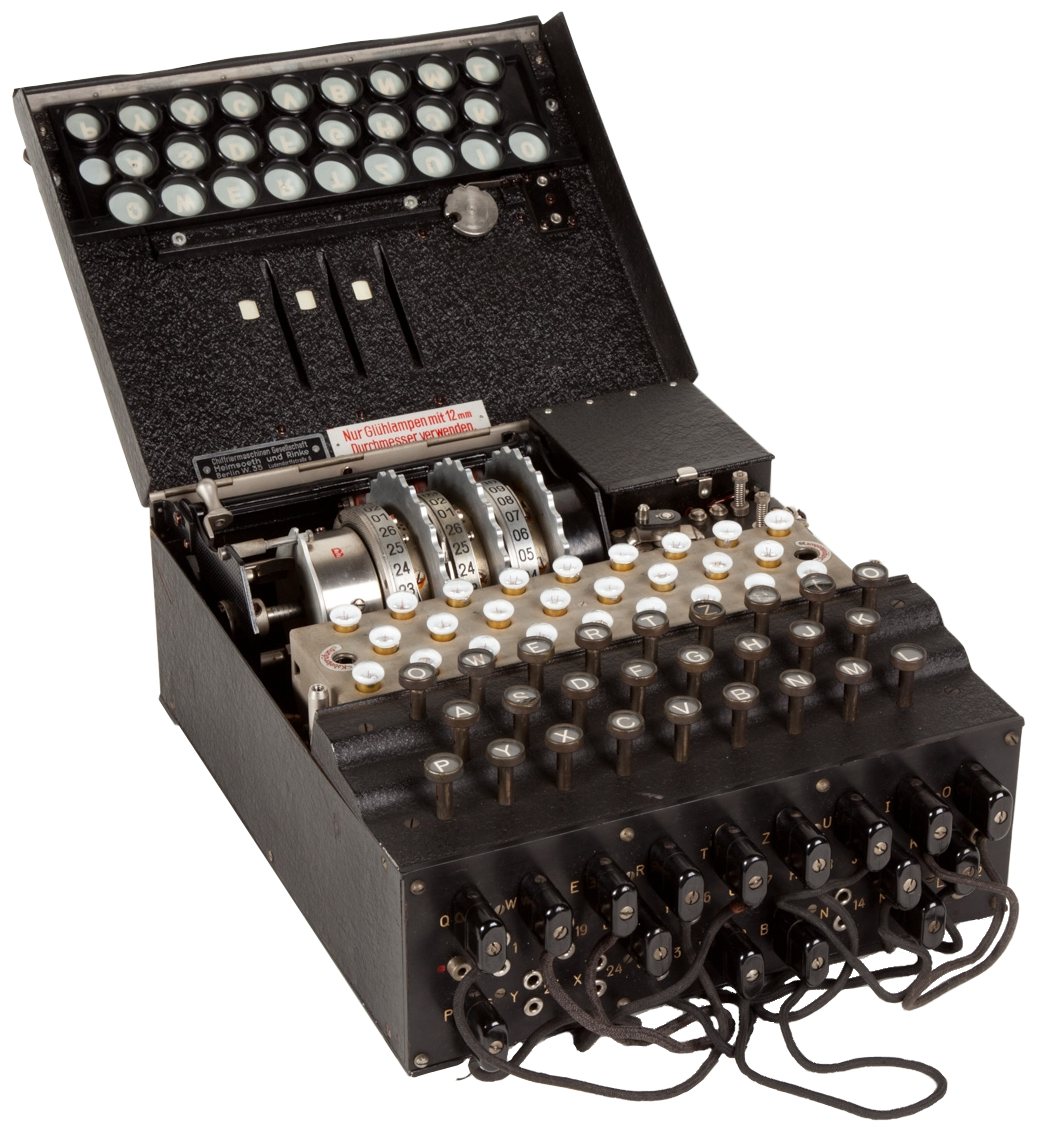
\includegraphics[width = 0.6\textwidth]{../assets/images/Enigma}
		\label{fig:Enigma}
		\caption{A German Enigma. Image: \href{https://de.wikipedia.org/wiki/Datei:Enigma_(crittografia)_-_Museo_scienza_e_tecnologia_Milano.jpg}{Alessandro Nassiri}}
	\end{figure}
\end{frame}
%%%

%%%
\begin{frame}{Encryption in the Age of the Computer}
		\begin{itemize}
			\item<1-> Electronics are much faster than mechanical parts
			\item<2-> Possibility to imagine hypothetical cipher machines
			\item<3-> Key difference: \\Numbers vs. Letters (ASCII)
		\end{itemize}
		\uncover<4->{
			\begin{table}
				\centering
				\resizebox{7cm}{!} {
					\begin{tabular}{c c c c c c c c c c c c c c c c c c c c c}
						\hline
						\textbf{A:}&&0&1&0&0&0&0&0&1& \hspace{0.4cm} &\textbf{N:}&&0&1&0&0&1&1&1&0\\
						\textbf{B:}&&0&1&0&0&0&0&1&0&&\textbf{O:}&&0&1&0&0&1&1&1&1\\
						\textbf{C:}&&0&1&0&0&0&0&1&1&&\textbf{P:}&&0&1&0&1&0&0&0&0\\
						\textbf{D:}&&0&1&0&0&0&1&0&0&&\textbf{Q:}&&0&1&0&1&0&0&0&1\\
						\textbf{E:}&&0&1&0&0&0&1&0&1&&\textbf{R:}&&0&1&0&1&0&0&1&0\\
						\textbf{F:}&&0&1&0&0&0&1&1&0&&\textbf{S:}&&0&1&0&1&0&0&1&1\\
						\textbf{G:}&&0&1&0&0&0&1&1&1&&\textbf{T:}&&0&1&0&1&0&1&0&0\\
						\textbf{H:}&&0&1&0&0&1&0&0&0&&\textbf{U:}&&0&1&0&1&0&1&0&1\\
						\textbf{I:}&&0&1&0&0&1&0&0&1&&\textbf{V:}&&0&1&0&1&0&1&1&0\\
						\textbf{J:}&&0&1&0&0&1&0&1&0&&\textbf{W:}&&0&1&0&1&0&1&1&1\\
						\textbf{K:}&&0&1&0&0&1&0&1&1&&\textbf{X:}&&0&1&0&1&1&0&0&0\\
						\textbf{L:}&&0&1&0&0&1&1&0&0&&\textbf{Y:}&&0&1&0&1&1&0&0&1\\
						\textbf{M:}&&0&1&0&0&1&1&0&1&&\textbf{Z}&&0&1&0&1&1&0&1&0\\
						\hline
					\end{tabular}
				}
				\caption{ASCII binary letters. Based on \cite{singh1999}}
		\end{table}}
\end{frame}
%%%

%%%
\begin{frame}{DES: Data Encryption Standard}
	\begin{itemize}
		\item<1-> Companies need a standardized approach
		\item<2-> Encryption Method ``Lucifer'' by Horst Feistel in early 1970s.
		\item<3-> Becomes ``Data Encryption Standard (DES)''
		\item<4-> Advantage: Standardization and security
		\item<5-> Disadvantage: Key distribution problem persists
	\end{itemize}
	\uncover<5->{
		\begin{figure}
			\centering
			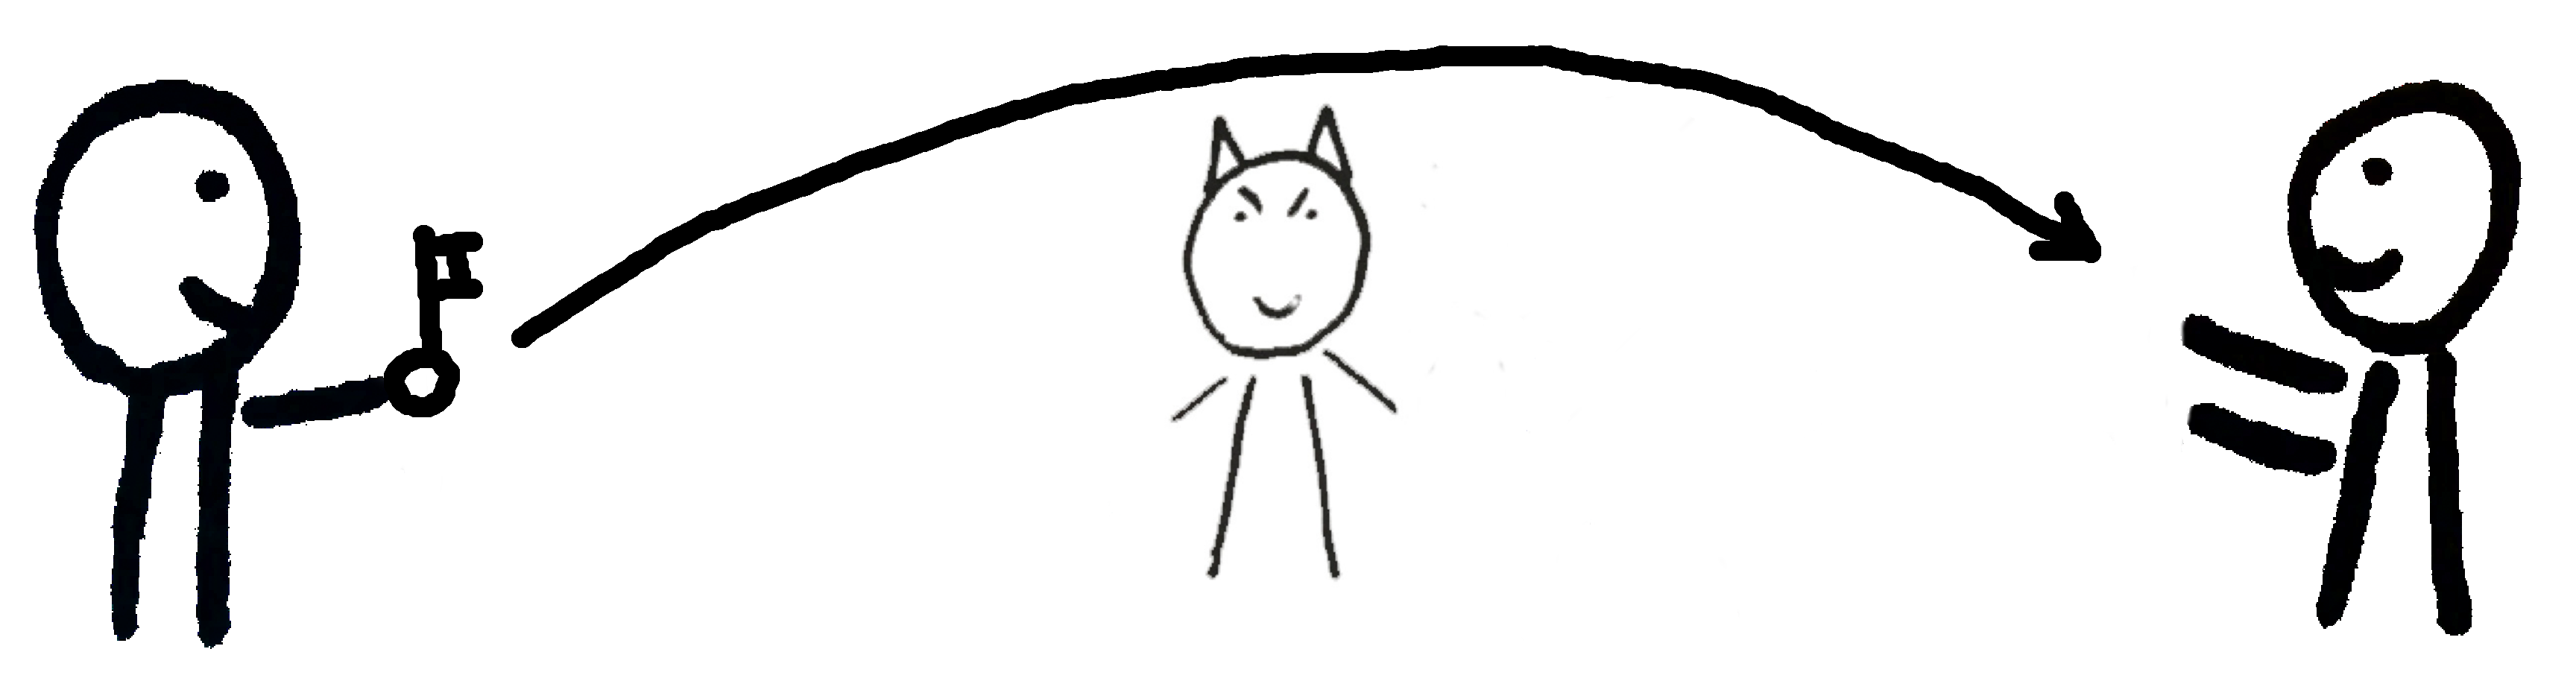
\includegraphics[width=0.8\linewidth]{../assets/images/drawing_key_exchange}
		\end{figure}
	}
\end{frame}
%%%

%%%
\begin{frame}%[allowframebreaks]
\frametitle{References and Recommended Reading}
	\bibliographystyle{amsplain}
	\bibliography{../assets/bib/refs}
\end{frame}
%%%

\end{document}